\begingroup
\setlength{\unitlength}{1bp}
\resizebox{.95\linewidth}{!}{\begin{picture}(1184,534)
\put(0,0){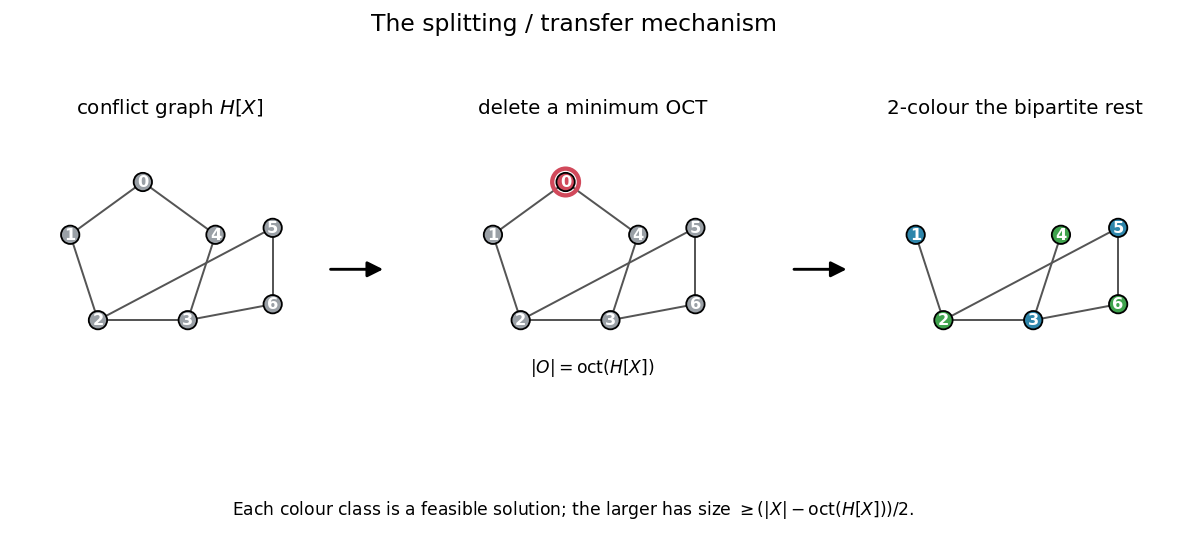
\includegraphics[width=1184bp,height=534bp]{figures/fig1_splitting_en.png}}
\put(0,480){\color{white}\rule{1184bp}{54bp}}
\put(592.0,507.0){\makebox(0,0){\raisebox{-.35\height}{\color{black}\fontsize{24}{26}\selectfont\sffamily El mecanismo de separación / transferencia}}}
\put(0,409){\color{white}\rule{345bp}{42bp}}
\put(172.5,430.0){\makebox(0,0){\raisebox{-.35\height}{\color{black}\fontsize{20}{22}\selectfont\sffamily grafo de conflictos \(H[X]\)}}}
\put(430,409){\color{white}\rule{335bp}{42bp}}
\put(597.5,430.0){\makebox(0,0){\raisebox{-.35\height}{\color{black}\fontsize{20}{22}\selectfont\sffamily eliminar una OCT mínima}}}
\put(840,409){\color{white}\rule{344bp}{42bp}}
\put(1012.0,430.0){\makebox(0,0){\raisebox{-.35\height}{\color{black}\fontsize{20}{22}\selectfont\sffamily 2-colorear el resto bipartito}}}
\put(0,0){\color{white}\rule{1184bp}{51bp}}
\put(592.0,25.5){\makebox(0,0){\raisebox{-.35\height}{\color{black}\fontsize{18}{20}\selectfont\sffamily Cada clase de color es factible; la mayor tiene tamaño \(\ge (|X|-\operatorname{oct}(H[X]))/2\).}}}
\end{picture}}
\endgroup
